\section{Технологический раздел}
Для написания программы необходимо определить, какие средства программной реализации требуется использовать. 
Для этого нужно привести перечень технологий и описать достоинства и недостатки конкретного выбора.

\subsection{Язык программирования}
Программный продукт реализуется на языке С++.
В научных вычислениях в последние годы все большее вниманиее обращается на язык с++ как основу для написаня простых в использовании и при этом выскоэффективных программных комплексов

Некоторые отличительные особенности языка C++:
\begin{enumerate}
	\item C++ содержит в себе все основные черты объектно-ориентированных языков программирования: наличие объектов и инкапсуляцию данных, наследование, полиморфизм и абстракцию типов;
	\item С++ широко использует указатели на переменные и функции, кроме того, поддерживает арифметику указателей, и тем самым позволяет осуществлять непосредственный доступ и манипуляции с адресами памяти; удобным средством для передачи параметров являются ссылки;
	\item Объем С++ невелик, так как практически все выполняемые функции оформлены в виде подключаемых библиотек, также С++ полностью поддерживает технологию структурного программирования и обеспечивает полный набор соответствующих операторов;
	\item Базовые типы данных совпадают с типами данных Ассемблера, на преобразования типов налагаются незначительные ограничения;
	\item С++ предлагает большой набор операций, многие из которых соответствуют машинным командам и допускают прямую трансляцию в машинный код, а их разнообразие позволяет выбирать различные наборы для минимизации результирующего кода;
\end{enumerate}

\subsection{Среды программирования}
\begin{enumerate}
	\item Clion
	\begin{enumerate}
		\item Clion - это современная кроссплатформенная IDE для С и С++ разработанная компанией JetBrains. Предоставляет помощь при написании кода с помощью Smart Completion. Позволяет генерировать шаблоны для классов. Быстрый просмотр документации и безопасный рефакторинг
	\end{enumerate} 
	\item VS Code
	\begin{enumerate}
		\item Visual Studio Code - редактор исходного кода, разработанный Microsoft для Windows, Linux и macOS. Позиционируется как «лёгкий» редактор кода для кроссплатформенной разработки веб- и облачных приложений. Включает в себя отладчик, инструменты для работы с Git, подсветку синтаксиса, IntelliSense и средства для рефакторинга. Имеет широкие возможности для кастомизации: пользовательские темы, сочетания клавиш и файлы конфигурации. Распространяется бесплатно, разрабатывается как программное обеспечение с открытым исходным кодом, но готовые сборки распространяются под проприетарной лицензией.
	\end{enumerate} 
\end{enumerate}

\subsection{Листинг}
\lstinputlisting{src/listings/ftp_client.c}

\subsection{Примеры работы программы}

\begin{figure}[H]
	\centering
	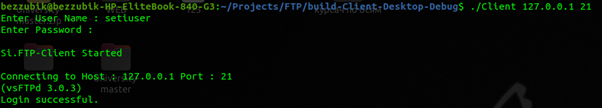
\includegraphics[width=0.7\linewidth]{src/img/6}
	\caption{Пример работы программы}
	\label{fig:6}
\end{figure}

\begin{figure}[H]
	\centering
	
\includegraphics[width=0.7\linewidth]{src/img/7}
	\caption{Пример работы программы}
	\label{fig:7}
\end{figure}

\begin{figure}[H]
	\centering
	
\includegraphics[width=0.7\linewidth]{src/img/7}
	\caption{Пример работы программы}
	\label{fig:8}
\end{figure}

\begin{figure}[H]
	\centering
	
\includegraphics[width=0.7\linewidth]{src/img/7}
	\caption{Пример работы программы}
	\label{fig:9}
\end{figure}

\begin{figure}[H]
	\centering
	
\includegraphics[width=0.7\linewidth]{src/img/7}
	\caption{Пример работы программы}
	\label{fig:10}
\end{figure}

